\section{Run Time Organization}

\subsection{Basics}

\begin{definition}[Machine Code]
    \textit{Machine Code} is a set of \textit{instructions} executed directly by CPUs.
\end{definition}

\begin{definition}[Assembly Code]
    \textit{Assembly} is a thin layer of abstraction on top of machine code, making it human readable.
    \begin{itemize}
        \item Can translate into object code or machine code via an \textit{Assembler}.
    \end{itemize}
\end{definition}

\begin{definition}[Run Time Organization]
    The execution of a user program is initially controlled by the Operating System (OS). When the program is launched,
    \begin{itemize}
        \item OS allocates memory for the program.
        \item Code is loaded into allocated memory.
        \item OS jumps to entry point (i.e. \texttt{main}).
    \end{itemize}
\end{definition}

\begin{definition}[C Program Memory Layout]
    A C program has the memory layout illustrated as follows:
    \begin{figure}[H]
        \centering
        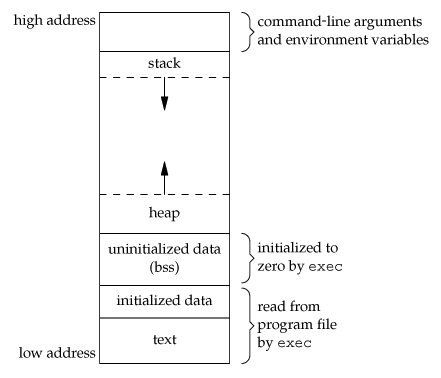
\includegraphics[height=20em]{figures/c-memory-layout.png}
        \caption{C program memory layout \cite{clayout}}
        \label{fig:c-memory-layout}
    \end{figure}
\end{definition}

\subsection{Procedure Activation}

\begin{definition}[Procedure Invocation / Activation]
    A procedure $P$ is \textit{invoked} or \textit{activated} when it is called, assuming
    \begin{enumerate}
        \item Sequential execution.
        \item Return address is immediately after call site.
    \end{enumerate}
\end{definition}

\begin{definition}[Lifetime of Activation of Procedure $P$]
    A procedure $P$ has the \textit{lifetime} of
    \begin{enumerate}
        \item All steps to execute $P$
        \item All steps within procedures called by $P$
    \end{enumerate}
\end{definition}

\begin{definition}[Lifetime of Variable $x$]
    A variable $x$ has the lifetime of the part of the execution for which $x$ is well defined dynamically. Note that this is not equivalent to the scope of variable $x$.
\end{definition}

\begin{definition}[Activation Tree]
    If procedure $P$ calls procedure $Q$, then $Q$ must return before $P$ is returned.
    \begin{itemize}
        \item The lifetimes of procedure activations are hence nested and recursive, allowing them to be represented by trees.
    \end{itemize}
\end{definition}

\begin{example}
    Given the procedures
    \begin{minted}{java}
class C
{
    public void foo()
    {
        // ...
        bar();
    }
    
    public void bar()
    {
        // ...
    }
    
    public static void main(String args[])
    {
        foo();
        bar();
    }
}
    \end{minted}
    
    Then the activation tree is given by
    \begin{figure}[H]
        \centering
        \begin{forest}
            [\texttt{main}
                [\texttt{foo}
                    [\texttt{bar}]
                ]
                [\texttt{bar}]
            ]
        \end{forest}
        \caption{Corresponding activation tree}
        \label{fig:example-activation-tree-normal}
    \end{figure}
\end{example}

\begin{remark}
    Since the activations are nested, a \textit{stack} could be utilized to track the currently active procedures.
\end{remark}

\begin{definition}[Activation Record]
    The information required to handle a procedure's activation is called an \textit{Activation Record} (AR) or a \textit{Stack Frame}.
    
    A generic activation record contains:
    \begin{enumerate}
        \item \textbf{Return values}.
        \item \textbf{Parameters}.
        \item \textbf{Control link} to previous activation record.
        \item \textbf{Return address} to caller.
        \item \textbf{Temporaries}.
        \item \textbf{Local variables}.
        \item \textbf{Access link} to additional data.
    \end{enumerate}
\end{definition}

\begin{remark}
    If a procedure $A$ calls procedure $B$, then the called procedure $B$'s stack frame consists of information from both $A$ and $B$. For instance, $B$'s stack frame need to keep track of the return address within $A$ in order to return control from $B$ to $A$ after $B$ completes its execution.
\end{remark}

\begin{definition}[Global Variable]
    A \textit{global variable} is a variable such that all references to it point to the same object, meaning that it cannot be stored on an activation record. This requires a fixed address to be assigned by the compiler.
\end{definition}

\begin{definition}[Dynamically Allocated Data]
    Any data which needs to have a lifetime longer than the procedure which created it cannot be kept within the creation procedure's activation record. This is resolved by allocating memory for storing the data on the \textit{Heap}.
\end{definition}

\begin{remark}
    Then, with reference to figure ~\ref{fig:c-memory-layout},
    \begin{itemize}
        \item \textit{Text} area contains the object code, fixed size and readonly.
        \item \textit{Initialized data} area contains data with fixed addresses, possibly writable and readable.
        \item \textit{Stack} contains activation records for each active procedure. Each stack frame usually has a fixed size with local variables.
        \item \textit{Heap} contains dynamically allocated data.
    \end{itemize}
    
    Notice that the \textit{stack} and \textit{heap} both grow in size dynamically as the program executes. It is thus important that they do not grow within each other causing memory access violations. This is resolved by having the \textit{stack} and \textit{heap} located at opposite ends of the memory and have them grow towards each other. A pointer of the lowest / highest address of the \textit{stack} and \textit{heap} is maintained respectively. When the \textit{stack} pointer meets the \textit{heap} pointer, there exists no more memory available for allocation.
\end{remark}

\subsection{Memory Management}

\begin{definition}[Garbage]
    A \textit{garbage} is any value that is no longer needed for execution by later parts of the program. Specifically, it refers to allocated memory which contains data that is no longer needed.
\end{definition}
